\chapter{Introduction}
\label{chapter:introduction}

%\emph{... \cite{example-article}}

\section{Background}
Over the years, many cities have gone through a transformation regarding surface and subsurface measures with the aim to mitigate and adapt to the consequences of climate change. Due to this transformation, the urban groundwater system became much more heterogeneous and complex in comparison with rural groundwater systems. Two aspects that characterize the behavior of he urban groundwater system includes surface sealing and systematic drainage of urban areas, resulting in surface drainage of precipitation to the sewage system, instead of replenishing the groundwater quantity through infiltration. The absence of infiltration into the soil is, however, compensated through a low actual evaporation [m/day] with surface sealing. Nonetheless, (ground)water nuisance occurs in urban areas, because the process of urbanisation does not include sustainable management and monitoring of the groundwater levels throughout the city (Ven et al., 2007).

Gemeente Rotterdam monitors an extensive groundwater monitoring network, consisting of approximately 2000 groundwater wells. The wells cover the entire municipal area of Rotterdam, reaching from urban to rural locations. The groundwater level in the monitoring wells gives insight into the groundwater level in the divided neighborhoods, but is not intended to be used for monitoring on household level. Monitoring groundwater is important to get an impression of fluctuations in groundwater levels in specific areas of attention within the municipality. Groundwater levels too high or too low are likely to result in problems on the topic of foundations and settlements, (ground)water nuisance in basements. The observed data by the municipality is used for civil technical measures and asset management. Monitoring wells that are constructed in public places are the city's responsibility. Because of the municipal duty to take care of the monitoring wells, it is of importance to monitor the groundwater level, but also to investigate whether the network density and the location of the monitoring wells are efficient enough to gain optimal results (Geul, 2022).


\section{Problem statement}

The degree of well coverage and monitoring methods differ between the neighborhoods of Rotterdam. One of the reasons is that Gemeente Rotterdam only investigates the coverage of a subarea when a well is expired; they determine the necessity of well replacement and if the new well can be placed on a more optimal and efficient location. Consequently, the number of groundwater wells has been stagnant throughout the years and it is not known if the current number of monitoring wells is the most suitable number to retrieve additional groundwater information (Geul, 2022). Since groundwater is an integral part of the hydrological cycle, it is key to monitor and anticipate the groundwater levels. Therefore, it is important to research the design of the network, analyze whether the network is optimal, and if monitoring wells need to be removed or reconstructed in a later stage (European Environment Agency, 2022). An insufficient groundwater monitoring network could lead to consequences for urban planning, infrastructure, and environmental pollution. An insufficient network might form an obstacle regarding Rotterdam’s ability to mitigate and adapt to climate change impacts such as increased precipitation variability. 
\newpage
\section{Research objective and questions}

Engaging the outlined research questions into a comprehensive approach, incorporating theoretical and empirical analysis. Even though the number of monitoring wells has been stagnant over the past years, the network is currently an actively monitored groundwater network. However, it is not known if the network is ideal yet. Therefore, the objective of the research study is to investigate the degree of optimization of the groundwater monitoring network of Rotterdam, see figure \labelcref{Research questions}.  \\

\begin{figure}[htbp]
    \centering
    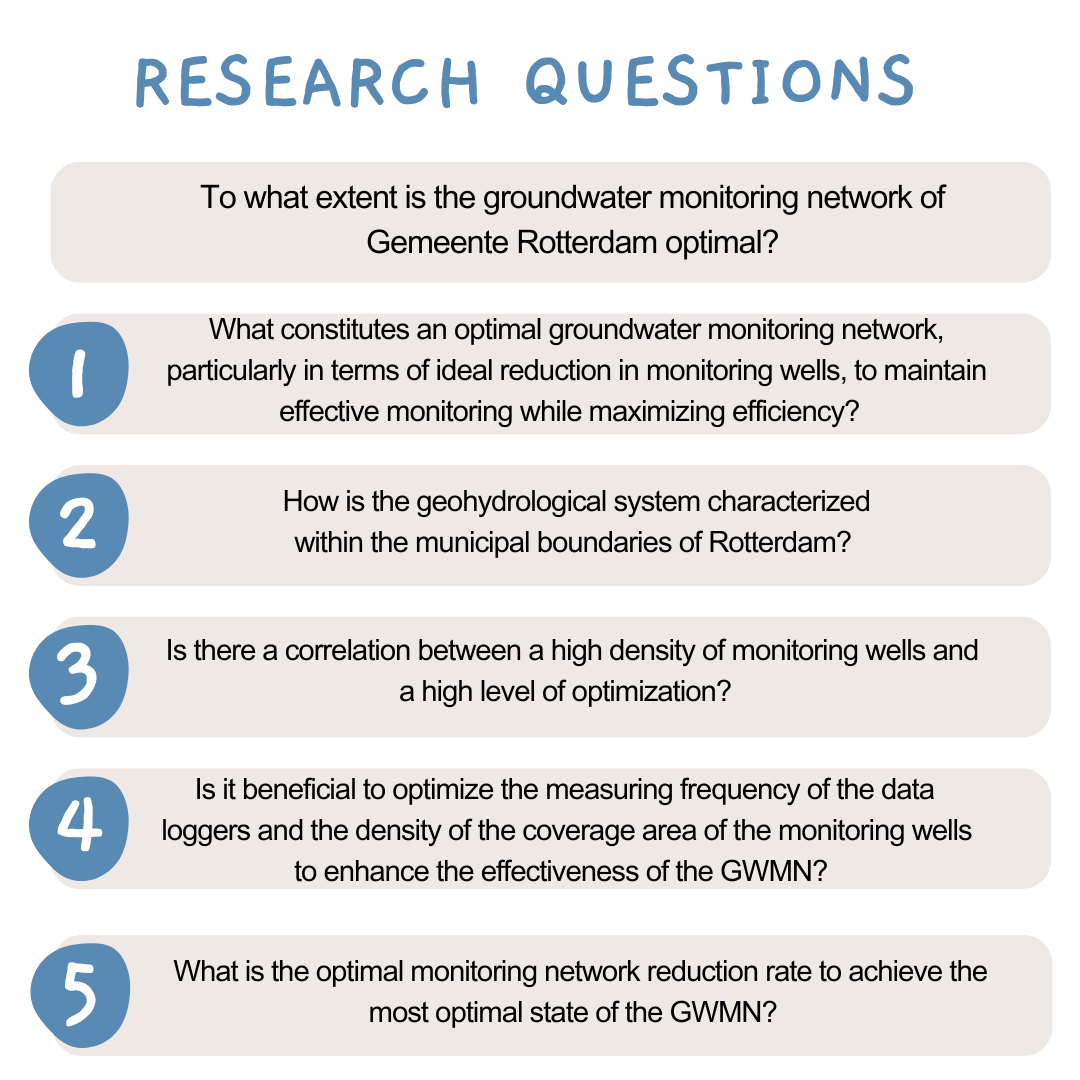
\includegraphics[width=0.75\linewidth]{figures/rq's-2.png}
    \caption{Main research question and five sub questions.}
    \label{Research questions}
\end{figure}
In the sub questions, the following topics are researched and discussed: 
\begin{itemize}
    \item The definition of optimal in the context of a groundwater monitoring network;
    \item Characteristics of the geohydrological system of the municipal area of Rotterdam through visualization of geological information;
    \item The correlation between network density and the degree of optimization;
    \item Advantages of optimizing the measuring frequency and coverage area of the monitoring wells;
    \item Comparison of reduction rates to determine the optimal reduction rate to achieve an optimal state of the GWMN.

\end{itemize}

\newpage

\section{Social and scientific relevance}

An overall assumption is made that the extent of optimization is low. Therefore, the study holds significant relevance as it delves into the aspects of groundwater monitoring networks within the municipal area of Rotterdam, particularly within an urban and industrial setting. The primary objective is to assess the level of optimization of the groundwater monitoring network in Rotterdam through the development of a generic QR factorization model. The outcomes of the research have the potential to serve as a valuable point of reference for other urban areas that face similar groundwater challenges. Accordingly, it is imperative to examine the GWMN to determine if sufficient and essential groundwater data are collected to make informed decisions for integrated groundwater management, because alignment between policy and execution is necessary to reach optimal groundwater management (Hoogvliet et al., 2020). The examination should include a critical review on the spatial distribution and network density of the GWMN as well as monitoring frequency. Overall, the study aspires to develop an innovative approach to monitor and enhance the optimization of Rotterdam’s GWMN, contributing to social and scientific advancements. 

\section{Scope}

The scope of this research study is limited by the following aspects: 
\begin{itemize}
    \item Only phreatic monitoring wells are included;
    \item Project monitoring wells within the study areas are not included; 
    \item The case study discusses Rozenburg and Heijplaat;
    \item Project period of 2010-2024 with the optimization approach for a period of 2020-2024;
    \item Development of a generic model.
\end{itemize}

\section{Reading guide}

The research study starts with an introducing chapter where the problem statement, research questions and relevance, and scope are the most important components. Followed by the chapter "Literature Review", multiple research methodologies are analyzed and compared in order to criticize whether the methodology could be applied to the current research study. At the end of the chapter, a short summary is written to determine which methodology is suitable. Moving on to the "Theoretical Background", where context is shared regarding the geological and hydrological context of the research area. As well as the current management and policy standards that are followed on local and national scale in The Netherlands. Starting with the "Research Methodology", the chapter starts with a short overview of the philosophy and approach that is considered. From there, a description of the research design is given, after which the method of data collection and preparation is introduced. In this subsection, there is already a separation between the case study areas of Rozenburg and Heijplaat. Followed by a description of the QR factorization methodology and the method of data analysis. At the end of the research methodology, an in-depth description is given of the geohydrological system of Rozenburg and Heijplaat. Continuing with the results of the "Research Methodology", a distinction is made between Rozenburg and Heijplaat, each with the subsections: QGIS and PROWAT, Pastas time series modeling, and QR factorization. The research study ends with an overview of the discussion points, mainly regarding the robustness of the model, and a concluding chapter, where the research questions are answered. An additional chapter "Future Recommendations" is present, because this chapter outlines the research limitations of the current study and should help designing practical and actionable suggestions for future research.












